\hypertarget{a00353}{}\section{Basic parameter update sequences}
\label{a00353}\index{Basic parameter update sequences@{Basic parameter update sequences}}
Sequence diagrams for some common parameter update scenarios. 

\hypertarget{a00353_advancedTopics_parameterUpdates_sequences_contents}{}\subsection{On this page}\label{a00353_advancedTopics_parameterUpdates_sequences_contents}
\begin{DoxyItemize}
\item \hyperlink{a00353_parameterUpdates_sequences_user}{User-\/generated update} \item \hyperlink{a00353_parameterUpdates_sequences_automation}{Automation playback} \item \hyperlink{a00353_parameterUpdates_sequences_initialization}{Initialization}\end{DoxyItemize}
\begin{DoxyNote}{Note}
To enable logging for these events at run time set {\ttfamily D\+T\+F\+\_\+\+A\+U\+T\+O\+M\+A\+T\+I\+O\+N=file@D\+T\+P\+\_\+\+L\+O\+W} in the \hyperlink{a00364}{Digi\+Trace} configuration file.
\end{DoxyNote}
\hypertarget{a00353_advancedTopics_parameterUpdates_sequences_notes}{}\subsubsection{Notes on threading for these sequences}\label{a00353_advancedTopics_parameterUpdates_sequences_notes}

\begin{DoxyItemize}
\item Calls from the host into \hyperlink{a00099}{A\+A\+X\+\_\+\+I\+Effect\+Parameters} may occur on any thread. In general, the only synchronization that is guaranteed for data model calls in these diagrams is that the call will follow whatever event is indicated as its trigger.
\item Calls from the host into \hyperlink{a00098}{A\+A\+X\+\_\+\+I\+Effect\+G\+U\+I} will occur on the main application thread unless indicated otherwise in the \hyperlink{a00098}{A\+A\+X\+\_\+\+I\+Effect\+G\+U\+I} documentation.
\item Host-\/driven updates to the algorithm context are always synchronized with the real-\/time processing thread
\end{DoxyItemize}\hypertarget{a00353_parameterUpdates_sequences_user}{}\subsection{User-\/generated update}\label{a00353_parameterUpdates_sequences_user}
This is the sequence of calls for a basic, unlinked parameter update triggered by the user. For this sequence, we assume that the edit was triggered by a G\+U\+I event.\hypertarget{a00353_parameterUpdates_sequences_updateSequences_user_highlevel}{}\subsubsection{High-\/level interface calls and events}\label{a00353_parameterUpdates_sequences_updateSequences_user_highlevel}

\begin{DoxyImage}
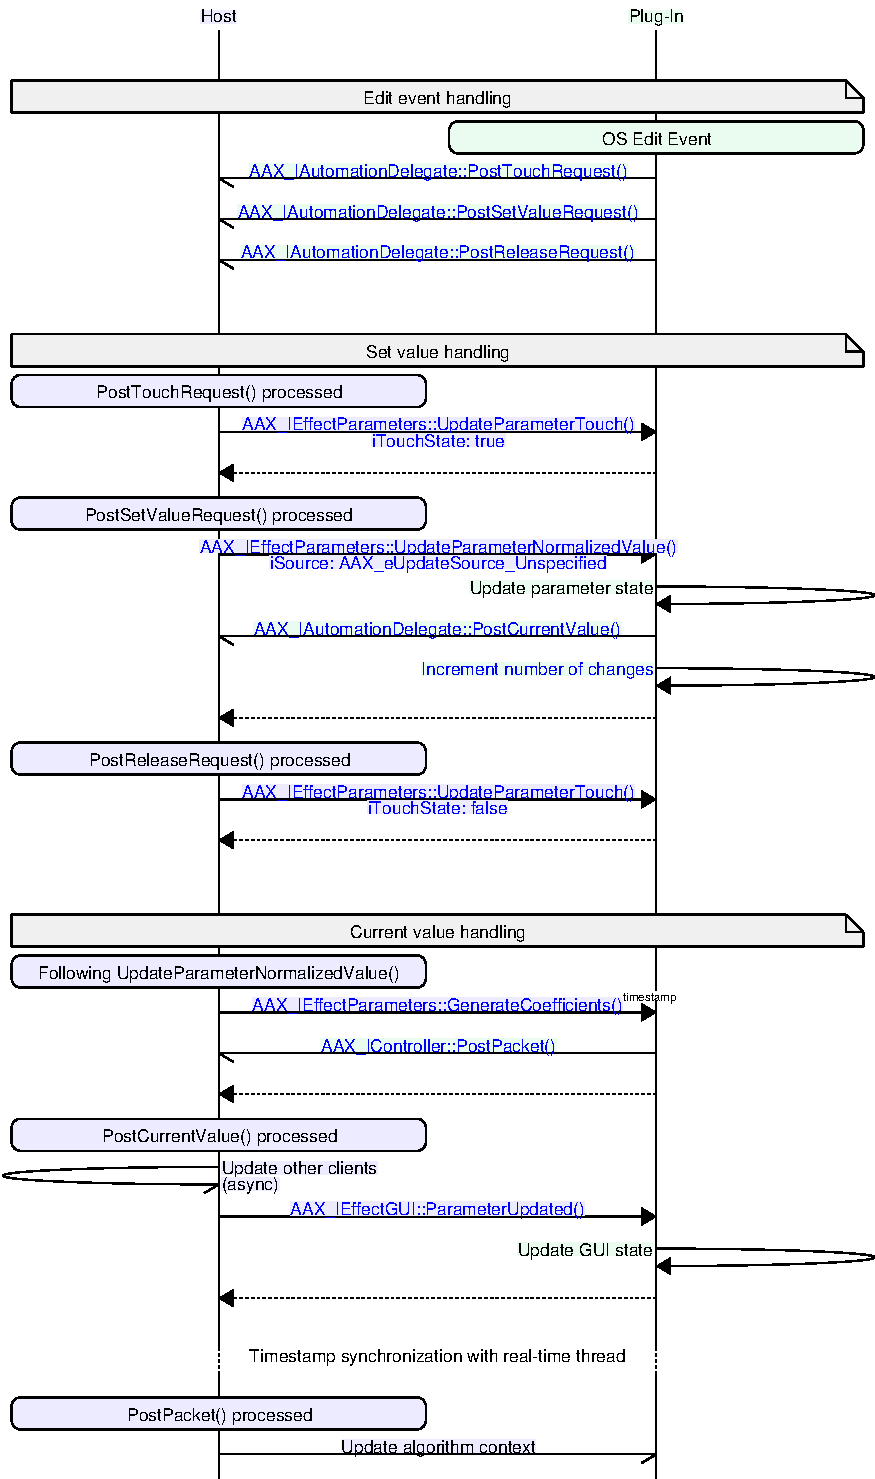
\includegraphics[width=\textwidth,height=\textheight/2,keepaspectratio=true]{msc_AAX_ParameterUpdate_GUI_HighLevel}
\caption{High-\/level sequence of interface calls and events for a parameter update following a user-\/generated edit}
\end{DoxyImage}
 \hypertarget{a00353_parameterUpdates_sequences_user_details}{}\subsubsection{Detailed sequence for default implementation}\label{a00353_parameterUpdates_sequences_user_details}
Note that this diagram assumes a G\+U\+I implementation that uses \hyperlink{a00061_a368b0f5a761d1eda4c41b420f153a077}{Set\+Parameter\+Normalized\+Value()}. The implementation could also use other parameter set methods, either in \hyperlink{a00099}{A\+A\+X\+\_\+\+I\+Effect\+Parameters} or directly on an \hyperlink{a00108}{A\+A\+X\+\_\+\+I\+Parameter}. The overall sequence would remain the same.


\begin{DoxyImage}
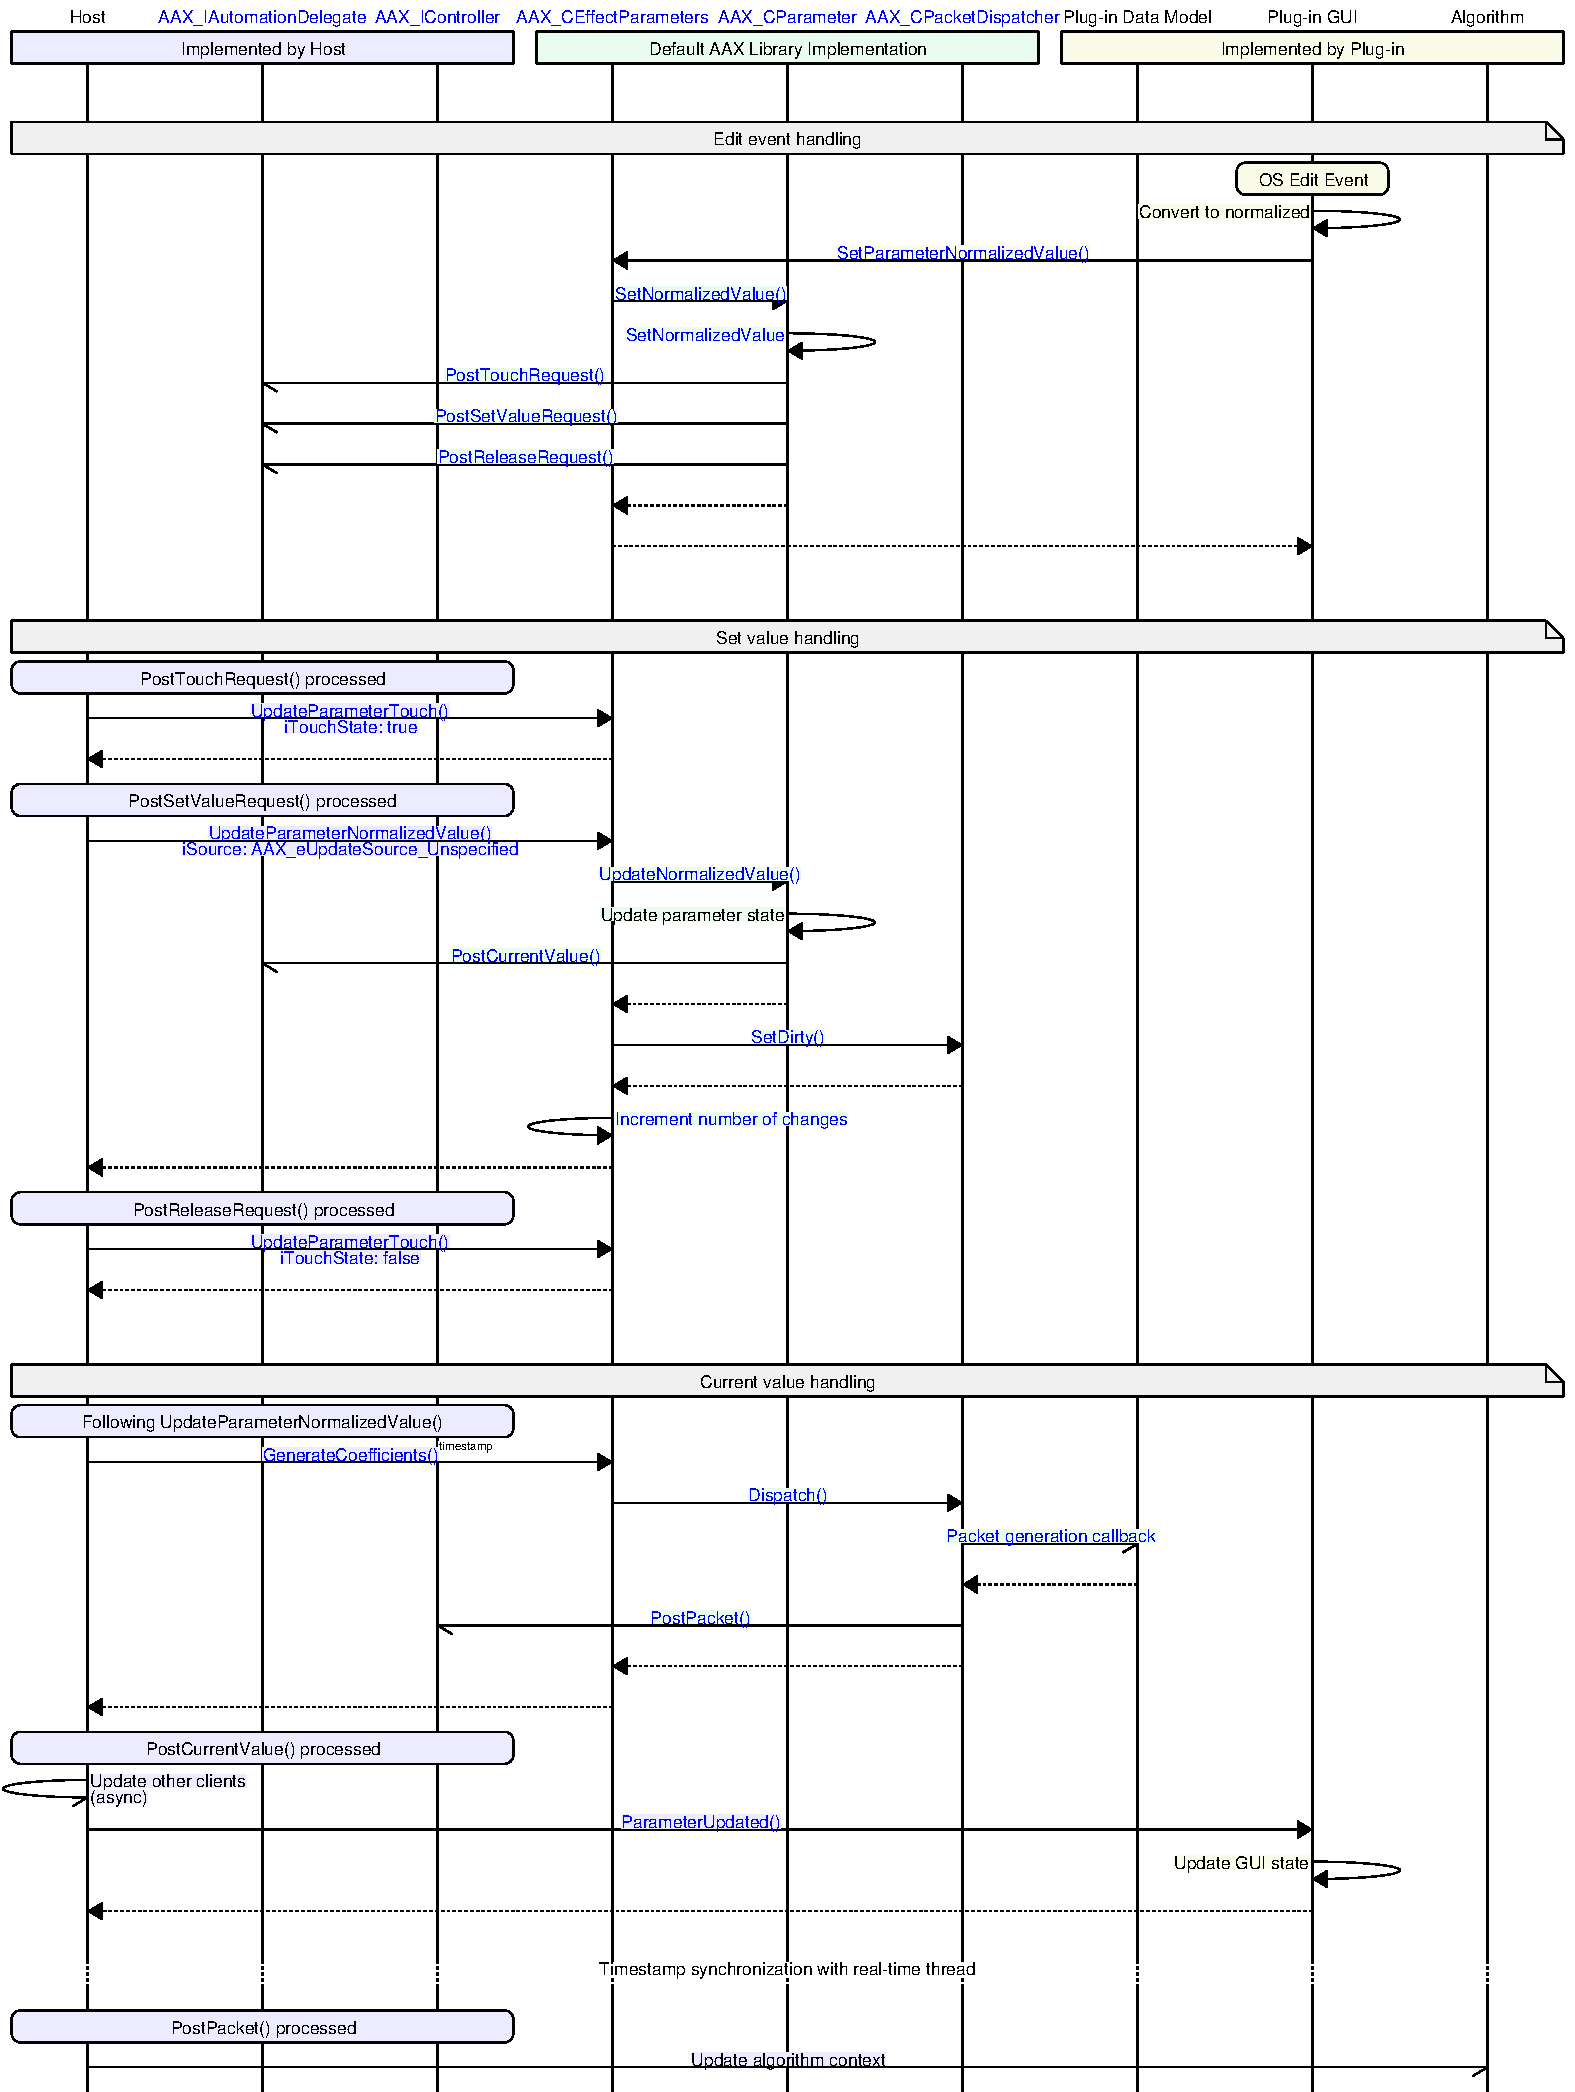
\includegraphics[width=\textwidth,height=\textheight/2,keepaspectratio=true]{msc_AAX_ParameterUpdate_GUI}
\caption{Detailed sequence of method calls and events for a parameter update following a user-\/generated edit on the plug-\/in G\+U\+I}
\end{DoxyImage}
 \hypertarget{a00353_parameterUpdates_sequences_user_controlsurface}{}\subsubsection{Updates from control surfaces}\label{a00353_parameterUpdates_sequences_user_controlsurface}
Updates from control surfaces are handled in exactly the same way. In this case, though, the parameter touch, set value, and release tokens are generated by the control surface.


\begin{DoxyImageNoCaption}
  \mbox{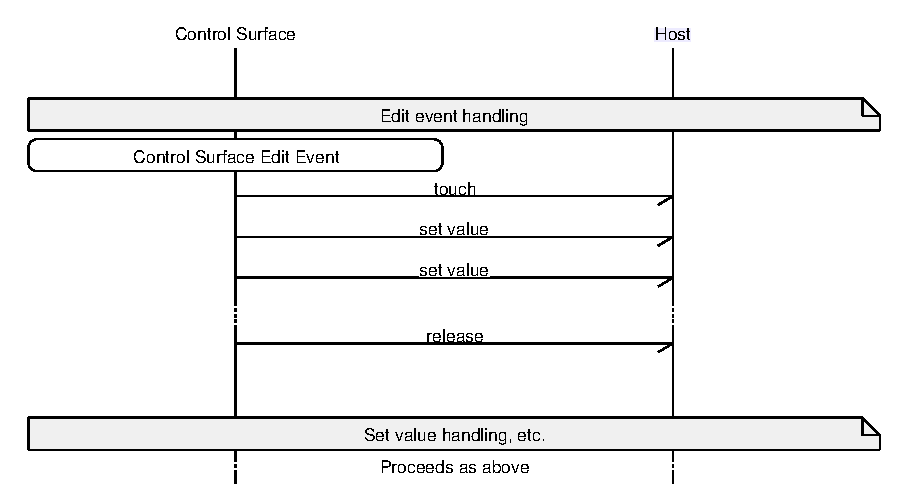
\includegraphics[width=\textwidth,height=\textheight/2,keepaspectratio=true]{inline_mscgraph_1}}
\end{DoxyImageNoCaption}
\hypertarget{a00353_parameterUpdates_sequences_automation}{}\subsection{Automation playback}\label{a00353_parameterUpdates_sequences_automation}
Automation playback handling is similar to the handling for user-\/generated parameter updates. However, parameters are never touched/released during automation playback. This allows touches from other clients, such as the G\+U\+I or control surfaces, to override the automation playback.


\begin{DoxyImage}
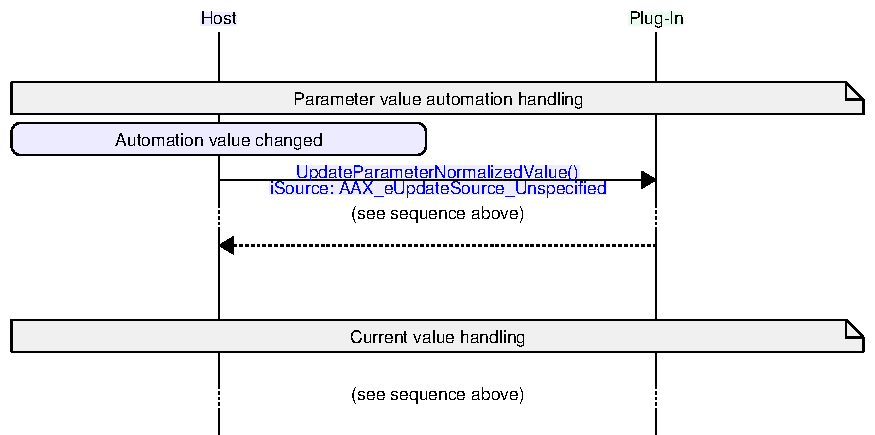
\includegraphics[width=\textwidth,height=\textheight/2,keepaspectratio=true]{msc_AAX_ParameterUpdate_Automation}
\caption{Sequence of method calls and events for playback of parameter automation}
\end{DoxyImage}
 \hypertarget{a00353_parameterUpdates_sequences_initialization}{}\subsection{Initialization}\label{a00353_parameterUpdates_sequences_initialization}
This is the sequence of calls for the initial parameter updates made during data model initialization. Steps that are redundant with sections of the \hyperlink{a00353_parameterUpdates_sequences_user_details}{standard user-\/generated update sequence} are elided.

\begin{DoxyRefDesc}{Todo}
\item[\hyperlink{a00382__todo000002}{Todo}]Update this section with information about default chunk setting, which is a separate step following the procedure described below.\end{DoxyRefDesc}



\begin{DoxyImage}
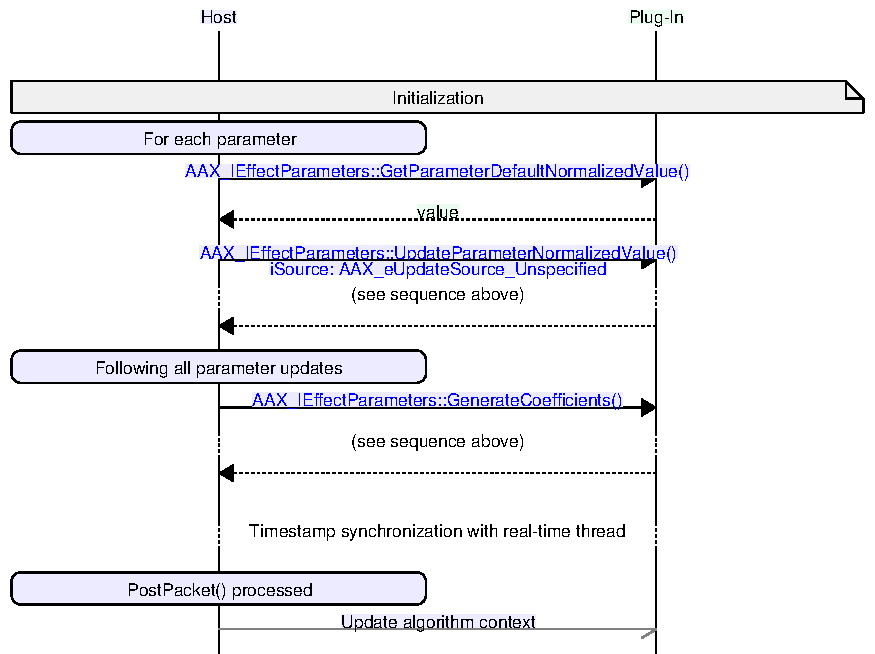
\includegraphics[width=\textwidth,height=\textheight/2,keepaspectratio=true]{msc_AAX_ParameterUpdate_Initialization}
\caption{Sequence of method calls and events for parameter updates at plug-\/in initialization}
\end{DoxyImage}
 Collaboration diagram for Basic parameter update sequences\+:
\nopagebreak
\begin{figure}[H]
\begin{center}
\leavevmode
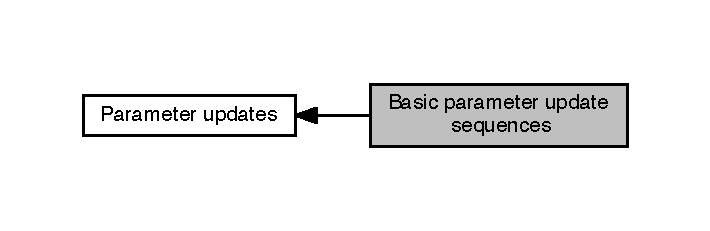
\includegraphics[width=341pt]{a00353}
\end{center}
\end{figure}
